\documentclass[a1paper,portrait,fontscale=0.43]{baposter}

\columnsep=70pt % This is the amount of white space between the columns in the poster
\columnseprule=3pt % This is the thickness of the black line between the columns in the poster

\usepackage{multicol} % Required for multiple columns
\setlength{\columnsep}{1.5em} % Slightly increase the space between columns
\setlength{\columnseprule}{0mm} % No horizontal rule between columns
\setlength{\multicolsep}{0mm} % No horizontal rule between columns

\usepackage[font=small,labelfont=bf]{caption}
\renewcommand{\figurename}{Fig.}

\usepackage{lmodern}

\usepackage[utf8]{inputenc} %unicode support
\usepackage[T1]{fontenc}

\selectcolormodel{rgb}

\graphicspath{{figures/}{../../schematics/svg/}} % Directory in which figures are stored

\newcommand{\compresslist}{%
  \setlength{\itemsep}{0pt}%
  \setlength{\parskip}{1pt}%
  \setlength{\parsep}{0pt}%
}

\newenvironment{boenumerate}
  {\begin{enumerate}\renewcommand\labelenumi{\textbf\theenumi.}}
  {\end{enumerate}}

\begin{document}

\definecolor{darkgreen}{cmyk}{0,0.90,0.74,0.28}
\definecolor{lightgreen}{cmyk}{0,0.90,0.74,0.28}
\definecolor{verdesinho}{rgb}{0, 51, 0}
%\definecolor{verdesinho}{rgb}{0, 51, 38}
\definecolor{cadet}{rgb}{0.33, 0.41, 0.47}
\begin{poster}
{
grid=false,
headerborder=open, % Adds a border around the header of content boxes
colspacing=1em, % Column spacing
bgColorOne=white, % Background color for the gradient on the left side of the poster
bgColorTwo=white, % Background color for the gradient on the right side of the poster
borderColor=black, % Border color
headerColorOne=cadet, % Background color for the header in the content boxes (left side)
headerColorTwo=lightgreen, % Background color for the header in the content boxes (right side)
headerFontColor=white, % Text color for the header text in the content boxes
boxColorOne=white, % Background color of the content boxes
textborder=roundedleft, %rectangle, % Format of the border around content boxes, can be: none, bars, coils, triangles, rectangle, rounded, roundedsmall, roundedright or faded
eyecatcher=true, % Set to false for ignoring the left logo in the title and move the title left
headerheight=0.15\textheight, % Height of the header
headershape=rounded, % Specify the rounded corner in the content box headers, can be: rectangle, small-rounded, roundedright, roundedleft or rounded
headershade=plain,
headerfont=\Large\bf\textsf, % Large, bold and sans serif font in the headers of content boxes
%textfont={\setlength{\parindent}{1.5em}}, % Uncomment for paragraph indentation
linewidth=2pt % Width of the border lines around content boxes
}
{}
%
%----------------------------------------------------------------------------------------
%	TITLE AND AUTHOR NAME
%----------------------------------------------------------------------------------------
%
{  
  {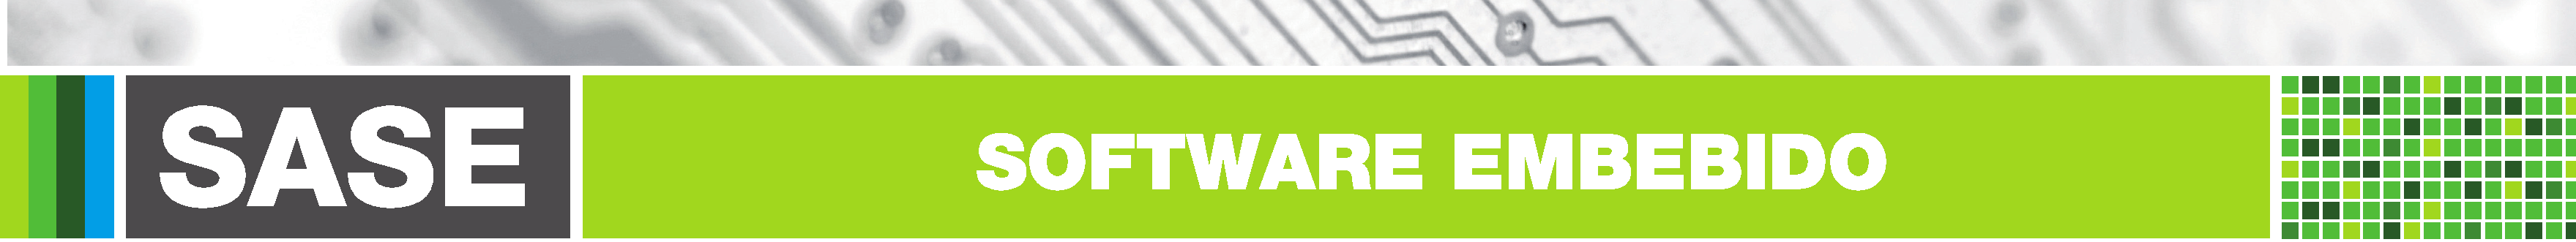
\includegraphics[trim=1.7cm 0 0 5cm, width=247mm]{software-embebido}\vspace{0.2em}}% SASE logo


  \huge\bf\textsf %Sans Serif  
  {Dynamic Reuse of Memory in 2D Convolution Applied to Image Processing}}
 % Poster title
% {\vspace{1em} Marta Stepniewska, Pawel Siedlecki\\ % Author names
% {\small \vspace{0.7em} Department of Bioinformatics, Institute of Biochemistry and Biophysics, PAS, Warsaw, Pawinskiego 5a}} % Author email addresses
{\sf\vspace{0.5em}\\
    Martin Casabella,
    Sergio Sulca,
    Ivan Vignolles,
    Ariel L. Pola
    \small{

      Department of Research and Development Fundacion Fulgor}\vspace{0.2em}
}
%{
\includegraphics[width=0.1\textwidth]{logo}} % University/lab logo

\headerbox{1. Introduction}{name=introduction,column=0,row=0, span=1}{
In this work, we explain the concept of dynamic reuse of BRAM in 2D convolution
and its complexity concerning implementation for parallel architectures. Moreover, we
propose a modular architecture, where it is easy to appreciate that when the
parallelism level increases, the complexity of BRAM increases linearly.
Given its local and two dimensional nature, 2-D Convolution is one of the most used image processing algorithms. 
Inherent parallelism of the image convolution algorithm can be exploited to increase the performance.
We focus our study on a more efficient design of 2D convolution technique
to reduce the usage of  FPGA resources.
}

\headerbox{2. Architecture Design}{name=screen,span=2,column=1}{ % To reduce this block to 1 column width, remove 'span=2'

The pre-processing consists of applying
a transformation to the image. Then the script divides the
image into batches and sends them through the UART port to the FPGA. In the FPGA a microprocessor receives the
information and transfers it to the convolution module using a 32 bits GPIO port. 
\begin{multicols}{2}
  \begin{center}
  \hfill\break
  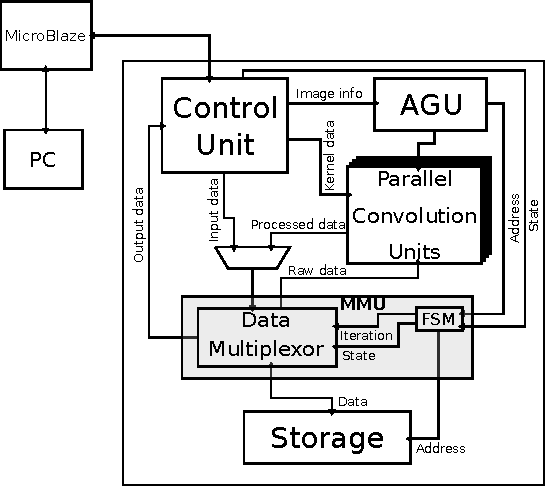
\includegraphics[width=\linewidth]{general}
  \captionof{figure}{Simplified block diagram of the convolution module implemented in FPGA.}
  \label{general}
  \end{center}
  \vfill\null
  \columnbreak
  The module is composed of the following units:
  \begin{description}
    \setlength{\itemsep}{1pt}
    \setlength{\parskip}{0pt}
    \setlength{\parsep}{0pt}
  \item[Control Unit] is the one in charge of handling the communication with
    the processor
  \item[Multiplier-Accumulator (MAC) Unit] executes the sum of the products of the kernel's coefficients with the pixels.
  \item[Address Generation Unit (AGU)] manages the memory addresses
  \item[Memory Management Unit (MMU)] decides how the values in memory are read and written.
  \item[Storage] is implemented with a set of columns of the FPGA's block RAM. 
  \end{description}
  When the operation ends, a notification is sent to the microprocessor, which
  gives the order to recover the processed batch from the module and sends it to
  the central processing unit (CPU). \end{multicols} Finally, the
post-processing stage combines the batches on the CPU.

\begin{multicols}{2}
  Given the nature of convolution operation there is an
  overlap between two MAC units inputs which produce adjacent columns. Consequently, despite $k$ input columns are needed per MAC unit, only $k+1$
  different input columns are needed for given two units. 
  Therefore, for $N$ MAC units, the number of required memory columns is reduced from $N \times k$ to $N+k-1$ 
  \setcounter{figure}{2}
  \begin{center}
  \hfill \break
  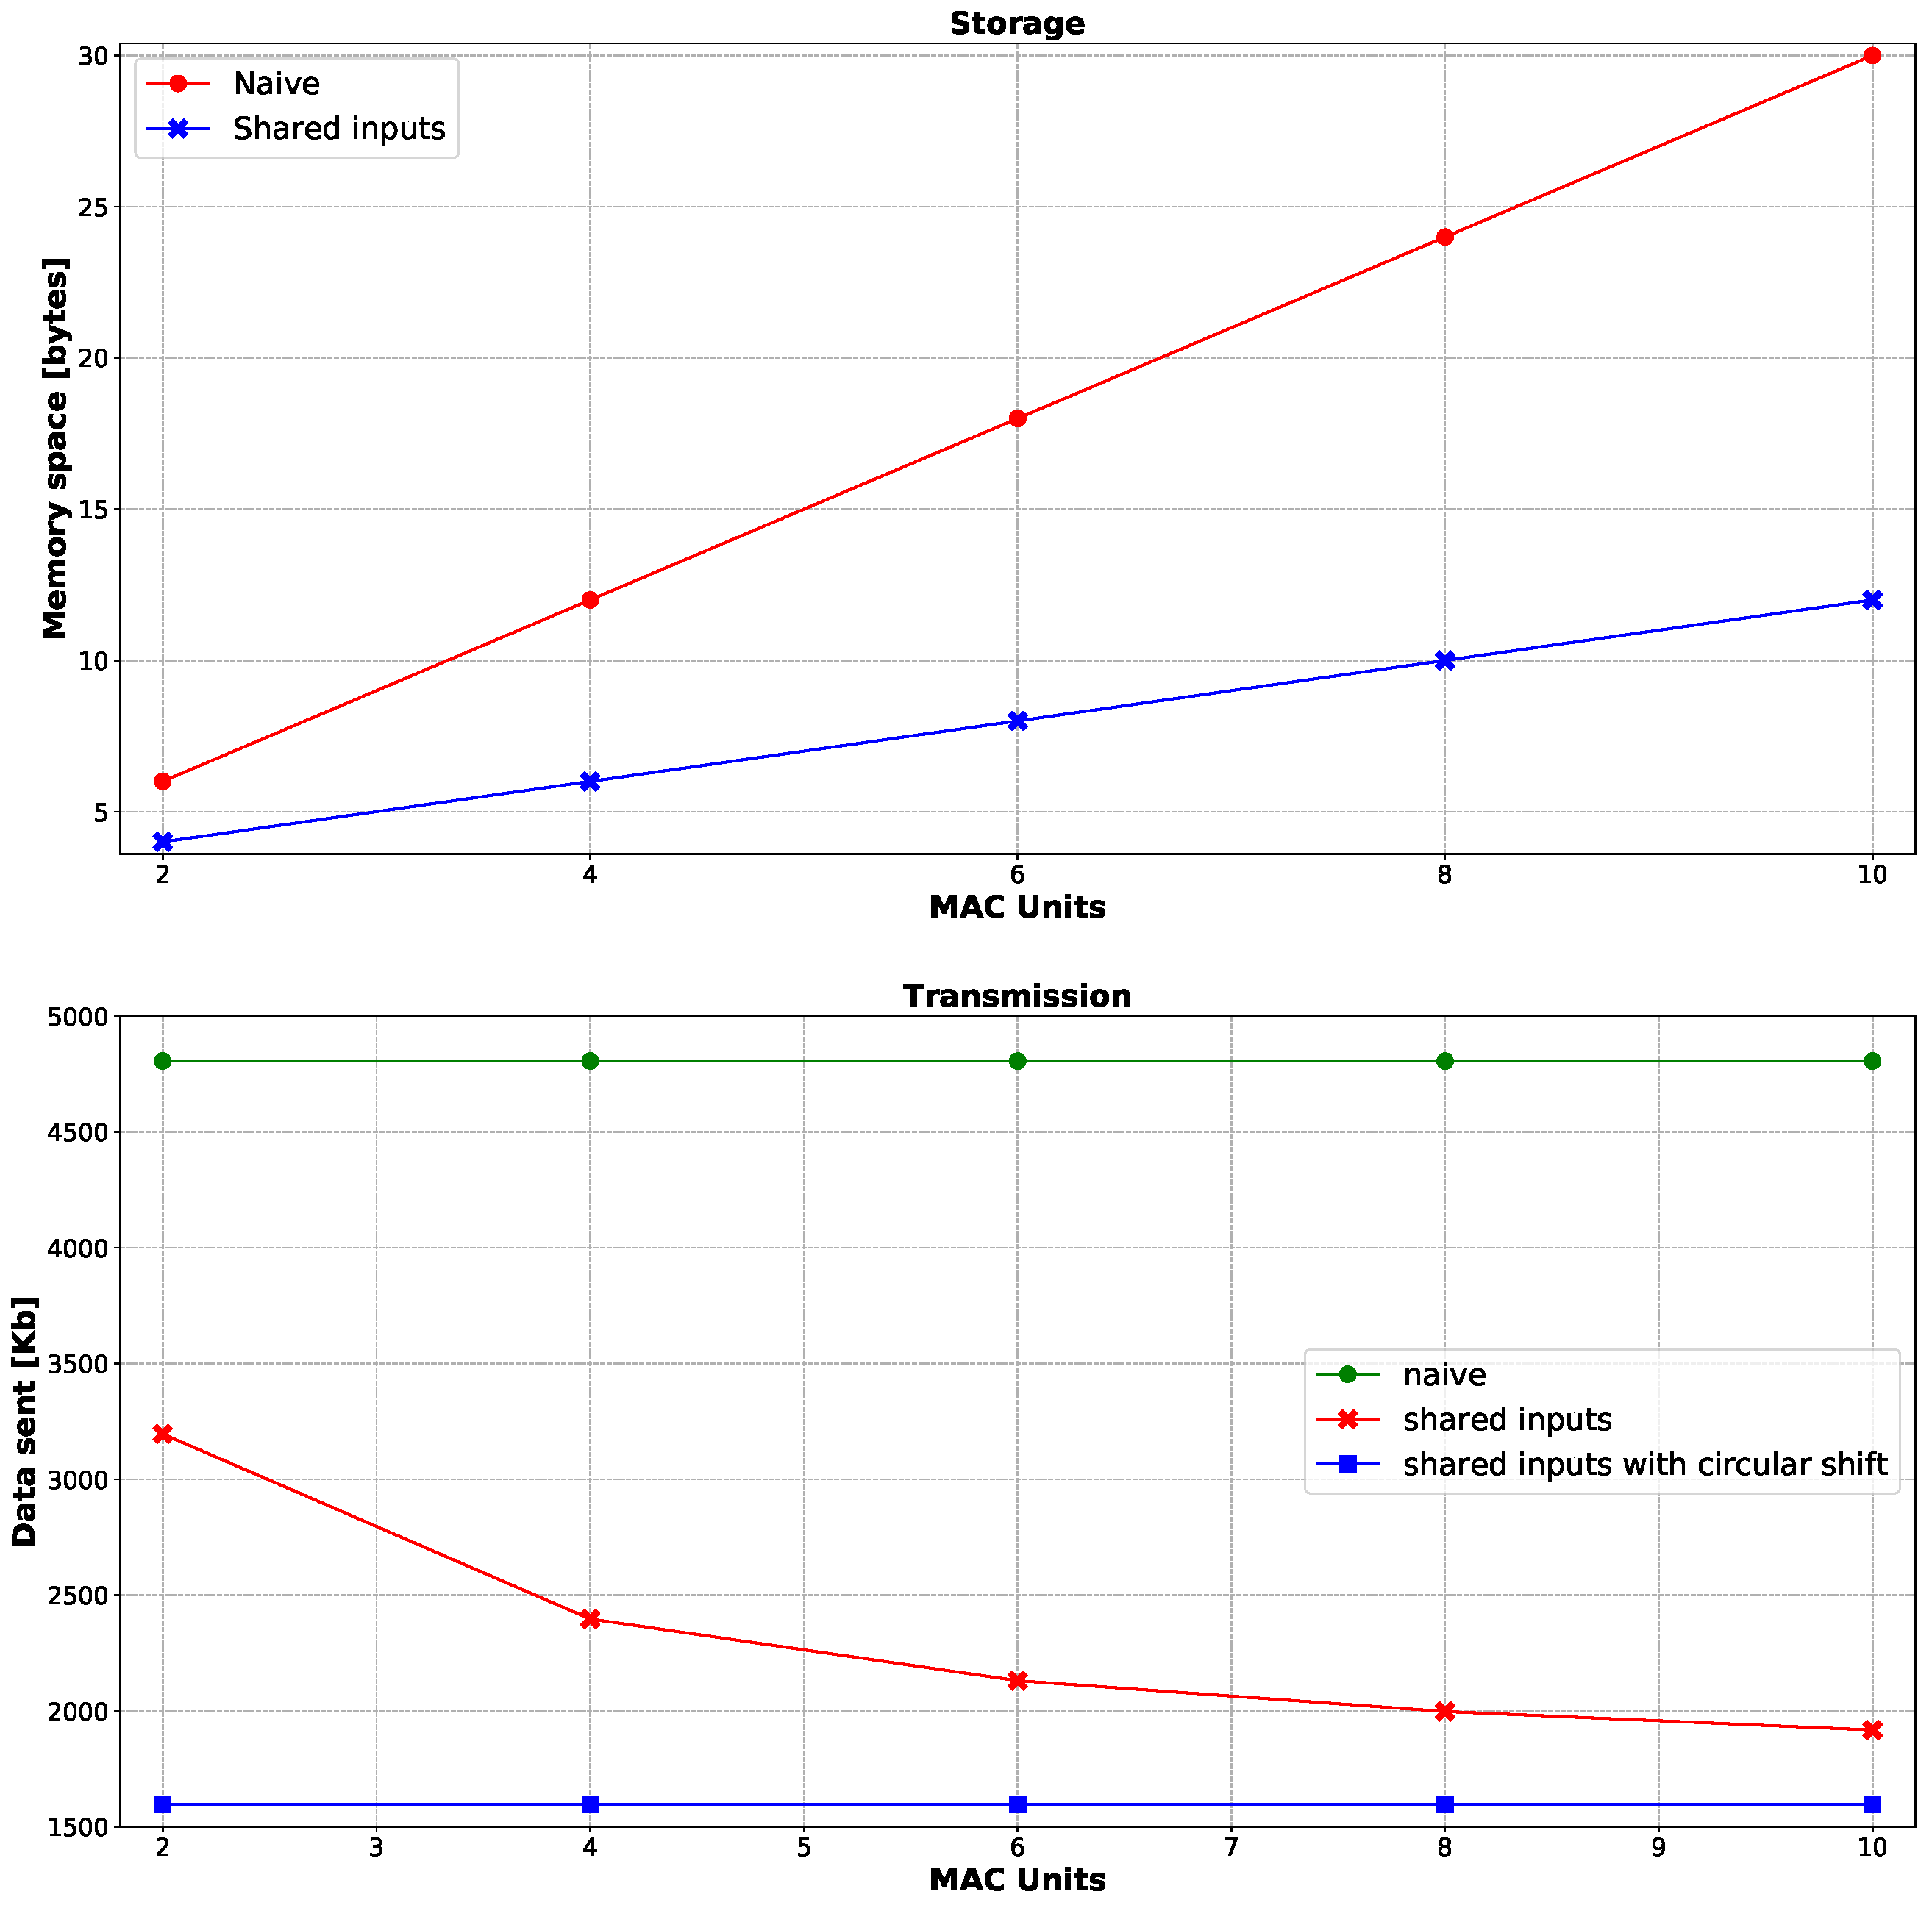
\includegraphics[width=\linewidth]{datas_mems}
  \captionof{figure}{Resources saving reusing data in memory for processing a
    $1600\times1024$ image and a $3\times3$ kernel.\\ Top - Amount of memory
    required. Bottom - Amount of transferred bytes}
  \label{dflow}
  \end{center}
  \vfill\null
  \columnbreak

  \setcounter{figure}{1}
  \begin{center}
  \hfill \break
  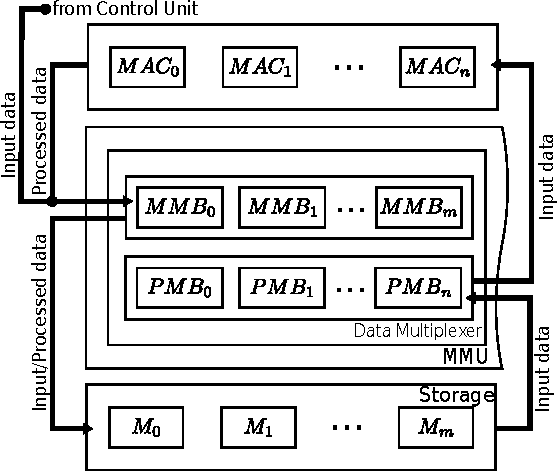
\includegraphics[width=\linewidth]{muxes}
  \captionof{figure}{The data flow between the MACs and the
  storage.}
  \label{dflow}
  \end{center}
  In order to reduce data transmission, repeated
  information is kept in memory and only the missing part of 
  the incoming batch is transmitted. This results in
  a circular shift by $N$ places, shifting memory columns possition associated with each
  MAC unit, in each iteration.
  The MMU has a set of multiplexers to route
  the incoming and outgoing data. The data multiplexer is
  conformed by two set of blocks: \textbf{memory multiplexer blocks (MMB)} and \textbf{processing multiplexer blocks (PMB)}. The MMB routes the
  raw data and the data from the MACs to a memory, whereas the PMB routes the data
  from the memories to a MAC.
\end{multicols}
}

\headerbox{3. Implementation and Results}{name=sea,span=1,column=0,below=introduction}{ % To reduce this block to 1 column width, remove 'span=2'

The design was implemented in a Xilinx Artix-35T FPGA (xc7a35ticsg324-1L) using
Xilinx Vivado Design Suite 2017.4 tools. A $100$ MHz reference clock
was synthesized.

Considering only convolution operation processing, i.e. not taking into account
the time needed to load the image into memory, one pixel per clock cycle ($100$ Mhz) is
obtained per instantiated MAC unit. Thus, throughput increases linearly with
parallelism degree. Table \ref{conv_tp} shows throughput obtained for
different parallelism degrees.
The architecture was synthesized for different degrees of parallelism.
Table~\ref{res_table} shows module and microprocessor complexity
on the FPGA with and without DSP respectively, measured by resource utilization. As a result, a linear increase is
shown according to parallelism. Due to implemented FPGA limitations a
parallelism up to 8 was achieved using DSP and up to 24 without DSP but with a
more intensive LUT usage.


\begin{center}
\begin{tabular}{|c|c|c|}
\hline
\textbf{Parallelism}  &    \textbf{Processing Speed [Mp/s]}  \\ \hline
        2             &                     200              \\ \hline
        4             &                     400              \\ \hline
        8             &                     800              \\ \hline
\end{tabular}           
\captionof{table}{Throughput achieved in convolution processing.}
\label{conv_tp}
\end{center}


\begin{center}
  \scalebox{0.75}{
\begin{tabular}{|c|c|c|c|c|c|}
  \hline
  & \multicolumn{3}{c|}{\textbf{With DSP [N](\%)}} & \multicolumn{2}{c|}{\textbf{Without DSP [N](\%)}} \\ \hline
  \textbf{P}  & \textbf{DSP}            & \textbf{LUT}        & \textbf{BRAM}         & \textbf{LUT}           & \textbf{BRAM}         \\ \hline
  2  & 20(22)         & 1845(9)    & 10(20)      & 3168(15)      & 10(20)         \\ \hline
  4  & 40(44)         & 2022(10)   & 11(22)      & 4627(22)      & 11(22)         \\ \hline
  6  & 60(67)         & 2175(10)   & 12(24)      & 6063(29)      & 12(24)         \\ \hline
  8  & 80(89)         & 2448(12)   & 13(26)      & 7756(37)      & 13(26)         \\ \hline
  10 & ---            & ---        & ---         & 9328(45)      & 14(28)         \\ \hline
  12 & ---            & ---        & ---         & 10917(52)     & 15(30)         \\ \hline
  24 & ---            & ---        & ---         & 20209(97)     & 21(42)         \\ \hline
\end{tabular}}           
\captionof{table}{Resource utilization table with and without DSP.}
\label{res_table}
\end{center}

\setcounter{figure}{3}
\begin{center}
  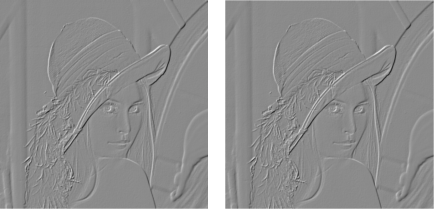
\includegraphics[height=3.45cm,keepaspectratio]{emboss_c2}
  \captionof{figure}{On the left, an image processed in a CPU using python and on the right the
  same image processed with the FPGA module.}
  \label{general}
\end{center}
}
	
\headerbox{4. Conclusions}{name=conclusion,column=1,below=screen,span=2,above=bottom}{
In this paper, we have presented the implementation of
two-dimensional convolution based on resource
efficiency and system parallelism. We implemented a whole image processing
system taking into account load stage, processing stage, and output stage.
Moreover, a relation between instantiated BRAM blocks and MAC units was
found in the presented architecture, which allows our system to work with different
parallelism degrees.
In addition, we optimized the use of memory resources implementing an algorithm
for memory operations and module synchronization. Performances and results show that resources utilization
concerning BRAM resources increase linearly, as desired. High throughput was
achieved in what processing is concerned.
}

\end{poster}
\end{document}
